\documentclass[../main.tex]{subfiles}


\begin{document}
	\section{Pokročilejší programování v jazyce Blocky}

	\subsection{Proměnné}
	Proměnné jsou krabičky, do kterých si robot může při běhu programu ukládat informace různých typů, jako např. čísla nebo slova. Jsou jedním z nejdůležitějších konceptů v programování ve všech jazycích a dovolují nám dělat řadu věcí, které bychom s našimi dosavadními znalostmi nemohli.

	K vytvoření proměnné stačí jít do sekce \textbf{Variables} v příkazové části, kliknout na \centerimage{\baselineskip}{Images/blocks/variable-create.png}, nějak jí pojmenovat a kliknout na \textbf{OK}. Jako jméno je vhodné zvolit něco, co odpovídá obsahu dané proměnné -- proměnná ukládající počet nárazů robota by se rozhodně neměla jmenovat \texttt{mrkvový\_guláš}!

	Po vytvoření libovolné proměnné budeme mít k dispozici příkazy, kterými s proměnnou budeme moci pracovat (k nalezení v části \textbf{Variables}):
	\begin{itemize}
		\blockVariableChange
		\blockVariableGet
		\blockVariableSet
	\end{itemize}

	 Příklad využití proměnných je např. tento program, který robota otáčí doleva o $1$ otáčku, poté o $2$, dále o $3$, apod. (s tím, že po jízdě vždy chvíli čeká):

	\begin{figure}[h!]
		\centering
		\begin{minipage}{0.5\textwidth}
			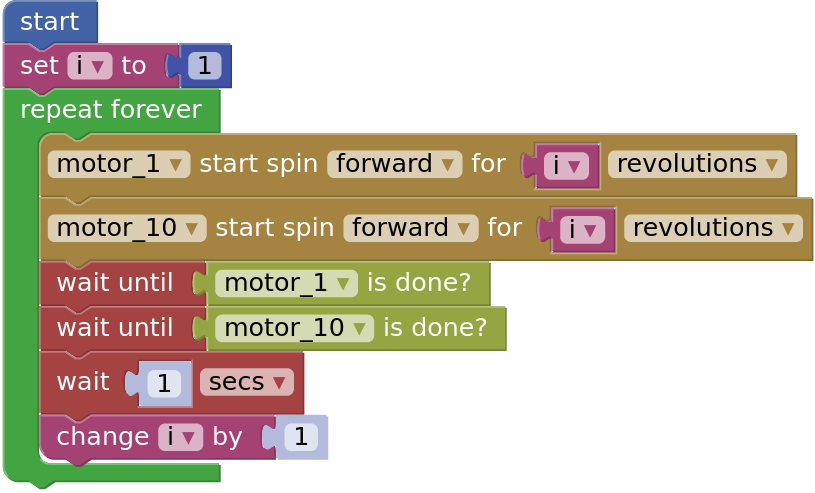
\includegraphics[width=\linewidth]{Images/05/variable-program.png}
		\end{minipage}
	\end{figure}

	Jména proměnných \texttt{i}, \texttt{j} a \texttt{k} jsou většinou používány pro to, když potřebujeme postupně procházet přes čísla $1, 2, \ldots$ (což právě v tomto příkladu potřebujeme).

	\subsubsection{Čísla}\label{cha:math}
	Čísla jsou jeden z typů informací, které do proměnné můžeme ukládat. Hodí se např. když chceme počítat, kolikrát jsme narazili, o kolik stupňů jsme se otočili nebo kolik ještě otáček chceme dělat. K tomu, abychom s nimi mohli pracovat, se nám budou hodit následující bloky (k nalezení v části \textbf{Math}):
  
	\begin{itemize}
		\blockMathOperation
		\blockMathTest
		\blockMathValue
		\blockMathConstant
		\blockMathRandom
	\end{itemize}

	\begin{question}
		Naprogramujte robota, aby jel otáčku dopředu a dozadu, poté dvě otáčky dopředu a dozadu, apod. (donekonečna).
	\end{question}

	\begin{solution}
		\begin{figure}
			\centering
			\begin{minipage}{0.5\textwidth}
				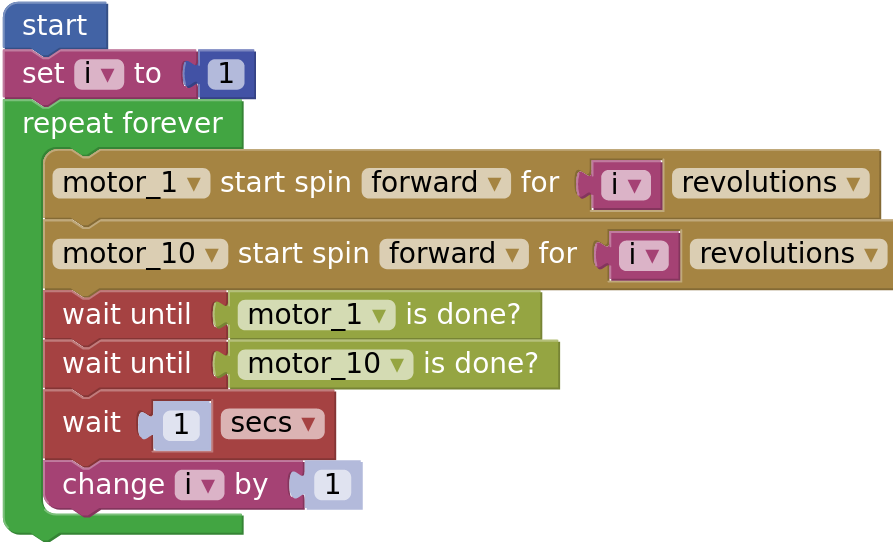
\includegraphics[width=\linewidth]{Images/05/solsim.png}
			\end{minipage}
		\end{figure}
	\end{solution}

	\begin{question}
		Naprogramujte robota, aby ujel vzdálenost, kterou mu na začátku programu uložíte do proměnné \texttt{vzdalenost} (v metrech). Všechny výsledky ke spočítání otáček/stupňů proveďte přes matematické bloky.
	\end{question}

	\begin{solution}
		\begin{figure}
			\centering
			\begin{minipage}{0.8\textwidth}
				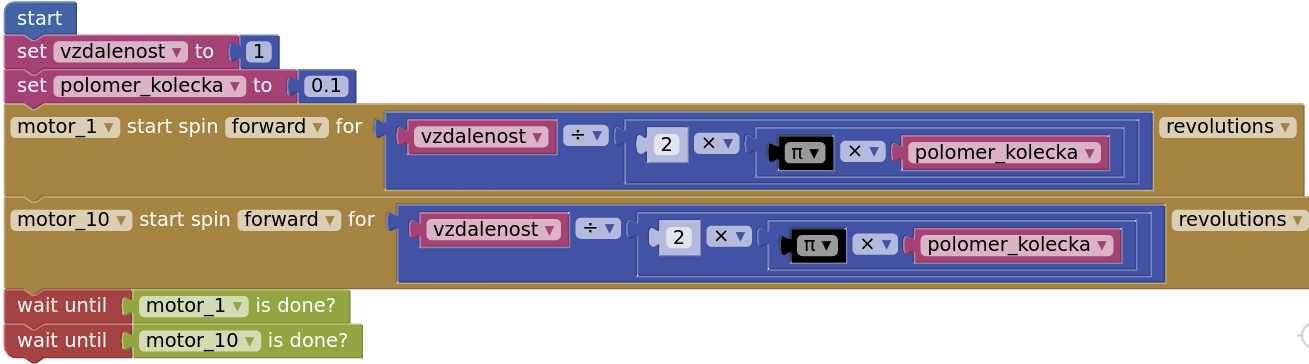
\includegraphics[width=\linewidth]{Images/05/solv.png}
			\end{minipage}
		\end{figure}
	\end{solution}

	\begin{question*}
		Naprogramujte samovyrovnávajícího robota, který bude stát na místě a dívat se rovně. Pokud do něj někdo strčí, tak se sám narovná do původního směru.
	\end{question*}

	\begin{solution}
		\begin{figure}
			\centering
			\begin{minipage}{0.8\textwidth}
				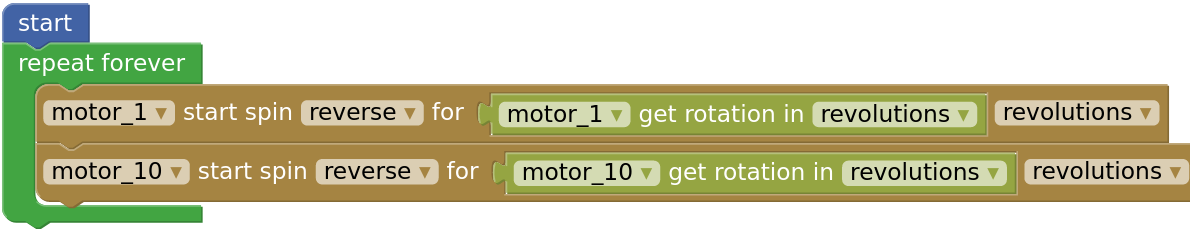
\includegraphics[width=\linewidth]{Images/05/solstay.png}
			\end{minipage}
		\end{figure}
	\end{solution}

	\begin{question*}
		Naprogramujte robota, aby jel do trojúhelníku, poté do čtverce, poté do pětistěnu, apod. (v jednom programu, donekonečna).
	\end{question*}

	\begin{solution}
		\begin{figure}
			\centering
			\begin{minipage}{0.8\textwidth}
				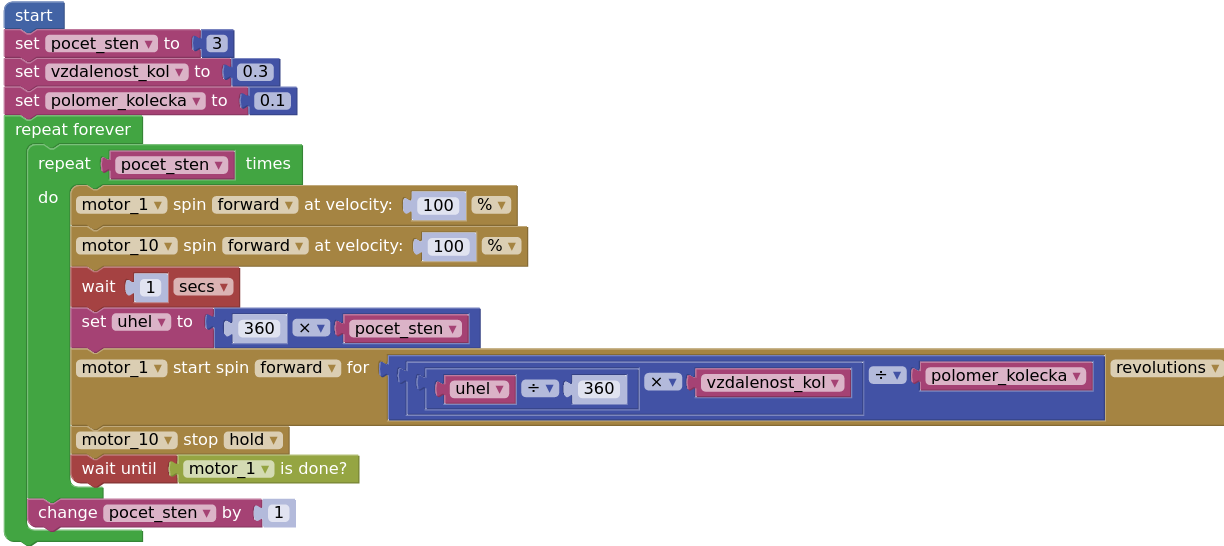
\includegraphics[width=\linewidth]{Images/05/soltri.png}
			\end{minipage}
		\end{figure}
	\end{solution}

	\subsubsection{Text}
	Druhým typem hodnot, se kterými se seznámíme, je text. Opět zde nepůjdeme příliš do detailu -- stačí nám vědět, že i text do proměnných ukládat umíme a můžeme s ním různými operacemi pracovat (k nalezení v částech \textbf{Text} a \textbf{VEX V5 Display}):

	\begin{itemize}
		\blockString
		\blockDisplayPrint
		\blockDisplayClear
	\end{itemize}

	\subsection{Funkce}
	Při programování složitějších programů v Blocky (a ostatních jazycích) se občas hodí mít „zkratky“ pro části kódu, které často používáme.

	Kdybychom měli například posloupnosti bloků pro otáčení doleva, otáčení doprava a jízdu rovně, a chtěli bychom naprogramovat robota pro jízdu v komplikovaném bludišti, tak není moc příjemné kopírovat stejných několik bloků za sebou.

	Právě k tomu se hodí funkce, které jsou pouze několik bloků za sebou, obalené do jednoho velkého bloku. Mohou mít navíc parametry -- proměnné, které se pro funkci nastaví, aby například robot ujel určitou vzdálenost, nebo se otočil o určitý úhel.

	K jejich vytváření a používání budeme používat následující bloky (k nalezení v části \textbf{Functions}):
	\begin{itemize}
		\blockFunctionDefinition
		\blockFunctionCall
	\end{itemize}

	\begin{question}
		Vytvořte tancujícího robota -- definujte funkce \texttt{doprava}, \texttt{doleva}, \texttt{dopředu} a \texttt{dozadu}, které posunou robota o malý kousek daným směrem. Poté použijte svou oblíbenou písničku a pomocí volání funkcí robota naprogramujte, aby do písničky tancoval!
	\end{question}

	\begin{question}\label{q:one}
		Vytvořte funkce
		\begin{itemize}
			\item \texttt{jed} s parametrem \texttt{vzdalenost}, kde robot ujede danou vzdálenost (v centimetrech).
			\item \texttt{otoc} s parametrem \texttt{uhel}, kde se robot otočí o daný úhel (ve stupních) doprava.
		\end{itemize}
	\end{question}

	\begin{solution}
		\begin{figure}
			\centering
			\begin{minipage}{0.7\textwidth}
				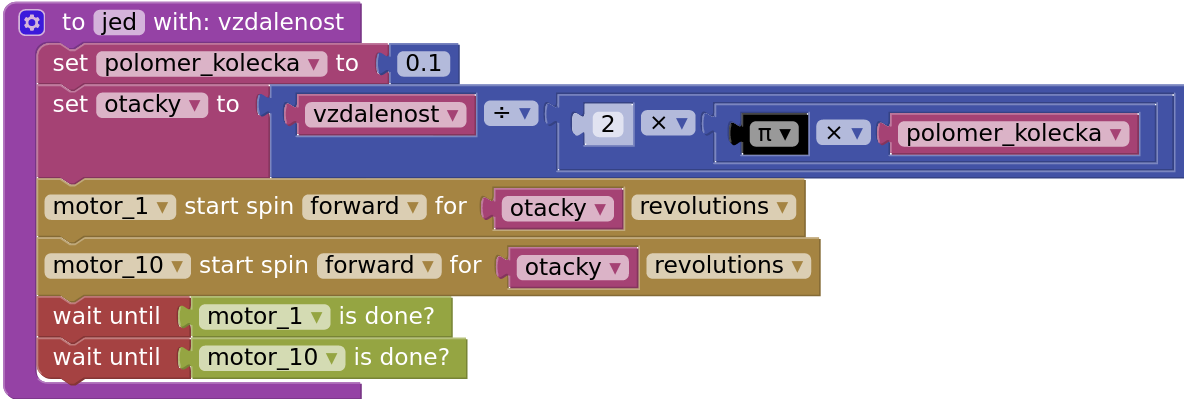
\includegraphics[width=\linewidth]{Images/05/fjed.png}
			\end{minipage}
		\end{figure}

		\begin{figure}
			\centering
			\begin{minipage}{0.7\textwidth}
				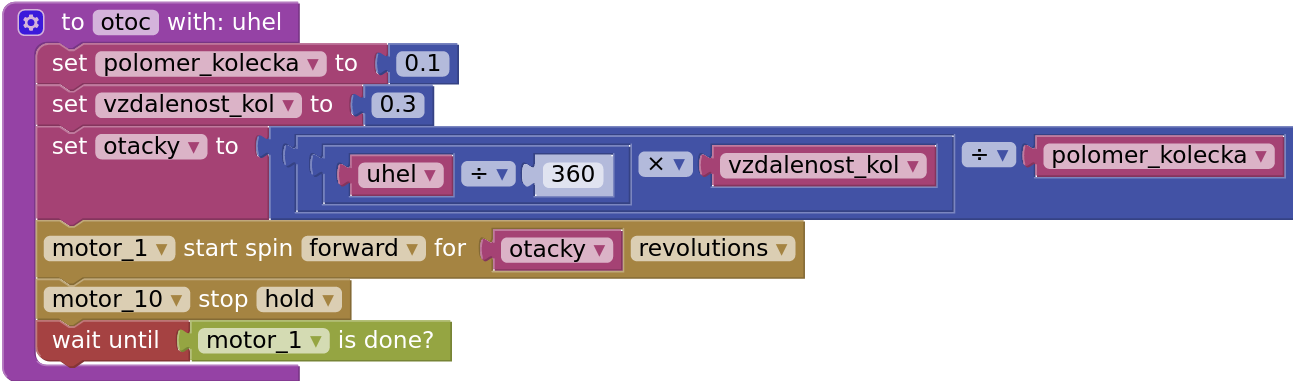
\includegraphics[width=\linewidth]{Images/05/fotoc.png}
			\end{minipage}
		\end{figure}
	\end{solution}

	\begin{question*}
		Vytvořte bludiště, které robot musí projet (kraje jde vymezit např. volnými kovovými díly stavebnice). K otáčení doprava/doleva použijte funkce z příkladu \ref{q:one}.
	\end{question*}

	\subsection{Druhý start}
	Při programování komplexnějších programů může být užitečné, kdyby robot dokázal vykonávat více bloků současně, např. když je potřeba současně řídit robota a vypisovat text na obrazovku.

	Blocky má pro tento případ přímočaré řešení -- pokud program obsahuje dva starty, tak se začnou vykonávat oba najednou. Příkladem je následující kód, který naprogramuje robota, aby jel dopředu a vypisoval u toho čísla od $1$ výše.

	\begin{figure}[h!]
		\centering
		\begin{minipage}{0.8\textwidth}
			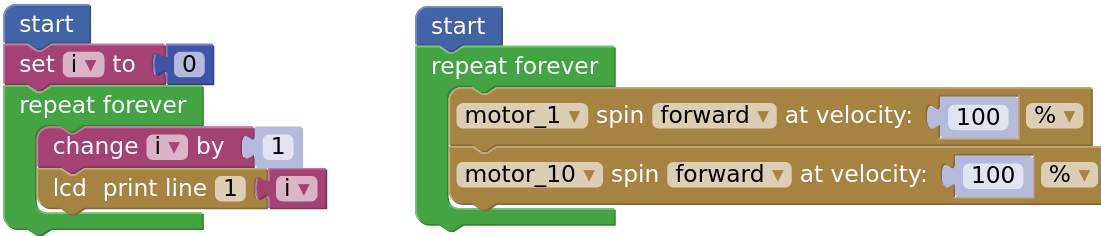
\includegraphics[width=\linewidth]{Images/05/2start.png}
		\end{minipage}
	\end{figure}

	\begin{question}
		Naprogramujte robota, aby jel donekonečna rovně a ukazoval při tom, kolik otáček již ujel (k nalezení v \textbf{VEX V5 Motors $\rightarrow$ Motor Detail}). Použijte k tomu dva starty.
	\end{question}

	\begin{solution}
		\begin{figure}
			\centering
			\begin{minipage}{0.5\textwidth}
				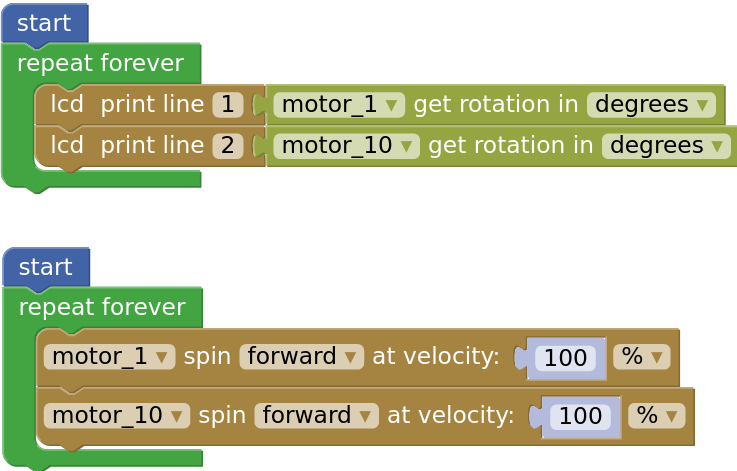
\includegraphics[width=\linewidth]{Images/05/solo.png}
			\end{minipage}
		\end{figure}
	\end{solution}

	\subsection{Podmínky}\label{cha:logic}
	Poslední, co nám zbývá, je vykonávat kód v závislosti na nějakých podmínkách (např. podle hodnoty nějaké proměnné). K tomu nám pomohou následující čtyři bloky (k nalezení v části \textbf{Logic}):
	\begin{itemize}
		\blockLogicIf
		\blockLogicIfElse
		\blockLogicComparison
		\blockLogicOperator
	\end{itemize}

	\begin{question*}
		Naprogramujte \href{https://en.wikipedia.org/wiki/Fizz\_buzz}{Fizz buzz} robota, který bude postupně na obrazovku vypisovat čísla (viz. předchozí část) od $1$ dále. Pokud je číslo dělitelné $3$, otočí se u toho doleva. Pokud $5$, tak doprava. Pokud jak $3$ tak $5$, tak provede oboje. K testování dělitelnosti použijte blok pro běžné matematické testy z části \ref{cha:math}.
	\end{question*}

	\begin{solution}
		\begin{figure}
			\centering
			\begin{minipage}{0.5\textwidth}
				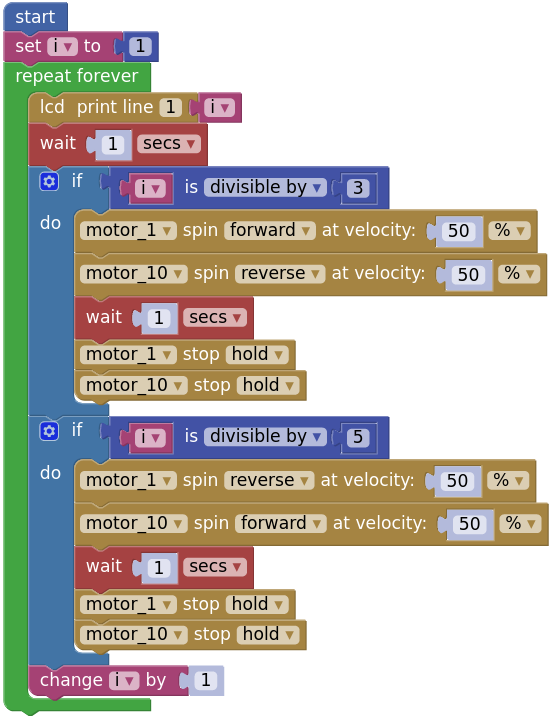
\includegraphics[width=\linewidth]{Images/05/solfb.png}
			\end{minipage}
		\end{figure}
	\end{solution}

\end{document}
